\documentclass[11pt,a4paper]{article}

\usepackage[utf8]{inputenc}
\usepackage[T1]{fontenc}
\usepackage{amsmath,amssymb}
\usepackage{booktabs}
\usepackage{geometry}
\usepackage{graphicx}
\usepackage{hyperref}
\usepackage{caption}
\usepackage{float}
\usepackage{enumitem}
\usepackage{multicol}

\geometry{margin=2.2cm}
\hypersetup{colorlinks=true,linkcolor=blue,citecolor=blue,urlcolor=blue}
\setlist{nosep,leftmargin=1.5em}
\captionsetup{font=small,skip=4pt}

\title{Transient Price Impact Estimation:\\
       Parametric and Non-Parametric Approaches}
\author{Anran Severac}
\date{\today}

\begin{document}
\maketitle

\begin{abstract}
\noindent
We estimate transient price impact on 50 US equities at 10-second
frequency over 2019, using two parametric models---the linear
Obizhaeva--Wang~(OW) and square-root Alfonsi--Fruth--Schied~(AFS)---and
a non-parametric binned extension with cross-stock regularisation.
The half-life~$H$ is selected by grid search; the OOS~$R^2$ surface is
flat in the 45--60\,min region, so a single universal $H^*\!=\!52.5$\,min
is adopted at negligible cost ($<\!0.0001$~$R^2$ for either model).
AFS dominates OW in out-of-sample~$R^2$.  Under apples-to-apples
pooled comparison the non-parametric estimator materially improves OW
($+5.9$\,pp) but is statistically indistinguishable from AFS,
confirming that the square-root form sits at the efficient frontier.
Cross-stock regularisation is immaterial in the data-rich headline
configuration but kicks in correctly under stress: shrinking training
windows from one month to two days raises the optimal $\gamma^*/n$
ratio from $0.16$ to $0.93$ and the OOS~$R^2$ gain
${\sim}14\times$---the estimator is regime-correct.
\end{abstract}

%=================================================================
\section{Data and Setup}

The panel consists of 50~US equities on a 10-second intraday grid for
all trading days in 2019 (12\,402 stock--days, 2\,341~bins each).  For
each stock--day we retain signed traded flow~$q_t$ (missing $\to$ 0) and
midprice~$P_t$ (forward/back-filled).  Flow is normalised by daily
volume $V=\sum_t|q_t|$ and scaled by intraday volatility
$\sigma=\mathrm{std}_t(r_t)$ so that impact coefficients are comparable
across stocks and days.

%=================================================================
\section{Methodology and Design Choices}

\subsection{Model Selection: OW vs.\ AFS}

Both models build an exponentially weighted impact state
$\bar I_{t+1}=(1{-}\beta)\bar I_t + \tilde q_t$
with $\beta=\ln 2/(H/10)$.
The only difference is the normalisation kernel applied to raw flow:
\[
  \text{OW:}\;\;\tilde q_t = \sigma\tfrac{q_t}{V},
  \qquad\qquad
  \text{AFS:}\;\;\tilde q_t = \sigma\,\mathrm{sgn}(q_t)\sqrt{|q_t/V|}.
\]
We fit both because they embody two competing hypotheses about the
shape of impact: linear in order size (OW) versus concave/square-root
(AFS).  Comparing them answers whether the well-documented concavity
of impact is material for out-of-sample prediction on this panel.

Over an explanation horizon $\tau{=}6$ bins (60\,s), we regress
midprice returns on changes in impact state:
$y_t = \alpha + \lambda\,x_t + \varepsilon_t$,
where $x_t=\bar I_t - \bar I_{t-\tau}$ and
$y_t=(P_t-P_{t-\tau})/P_{t-\tau}$.
All OLS is performed on additive sufficient statistics
$(S_x,S_y,S_{xx},S_{yy},S_{xy},n)$, enabling fast monthly aggregation.

The key computation functions follow this pipeline:

\smallskip
\noindent
\texttt{impact\_state}$(Q, \sigma, V, H, \text{model}) \to \bar I$
\;\;$\longrightarrow$\;\;
\texttt{impact\_regression\_statistics}$(\bar I, \tau, P) \to (x,y,\text{suff.\ stats})$
\;\;$\longrightarrow$\;\;
\texttt{ols\_from\_sums / r2\_from\_sums}

\subsection{Half-Life Selection}
\label{sec:halflife}

The half-life $H$ governs how quickly past order flow is ``forgotten''
by the market.  Rather than prescribing a fixed value (e.g.\ 60\,min as
in standard course materials), we treat $H$ as a hyperparameter and
select it empirically.  This is an important choice: $H$ conflates with
$\lambda$ in the regression, so fixing $H$ arbitrarily biases the
estimated impact coefficient.

\paragraph{Grid search procedure.}
For each $H\in\{5,10,20,30,45,60,90,120,180\}$\,min and each model
type, we run the full rolling OLS across 10~windows and record the
\emph{mean OOS~$R^2$} (averaged over all stocks and windows).

\paragraph{Why mean OOS~$\boldsymbol{R^2}$?}
We optimise mean rather than, say, median OOS~$R^2$ because the
per-stock OOS~$R^2$ distribution is approximately symmetric with no
heavy tails, so the mean is a stable summary.  Since our downstream use
of the model weights all stocks equally, mean~$R^2$ directly measures
the quantity we care about.

\paragraph{Results and universal $\boldsymbol{H^*}$.}
Figure~\ref{fig:halflife} and Table~\ref{tab:grid} show that OW peaks
at $H^*_\text{OW}=60$\,min and AFS at $H^*_\text{AFS}=45$\,min.
Crucially, the OOS~$R^2$ curve is essentially \emph{flat} in the
45--60\,min region: both models lose $<0.001$ in $R^2$ anywhere in that
range.  We therefore adopt a single universal half-life equal to the
midpoint:
$H^*=(3600+2700)/2=3150$\,s $\approx52.5$\,min.

The choice is supported empirically: forcing OW to use $H{=}45$\,min
(AFS's optimum) costs $<\!0.0001$ in OOS~$R^2$ relative to its own
optimum at $60$\,min, and forcing AFS to use $H{=}60$\,min costs
$<\!0.0001$ relative to its optimum at $45$\,min---both differences are
in the fourth decimal place, well below other sources of variation.
Adopting the midpoint $H^*=52.5$\,min therefore incurs no measurable
performance loss for either model, while providing the common impact
state required by the non-parametric extension
(Section~\ref{sec:np}).

\begin{figure}[H]
  \centering
  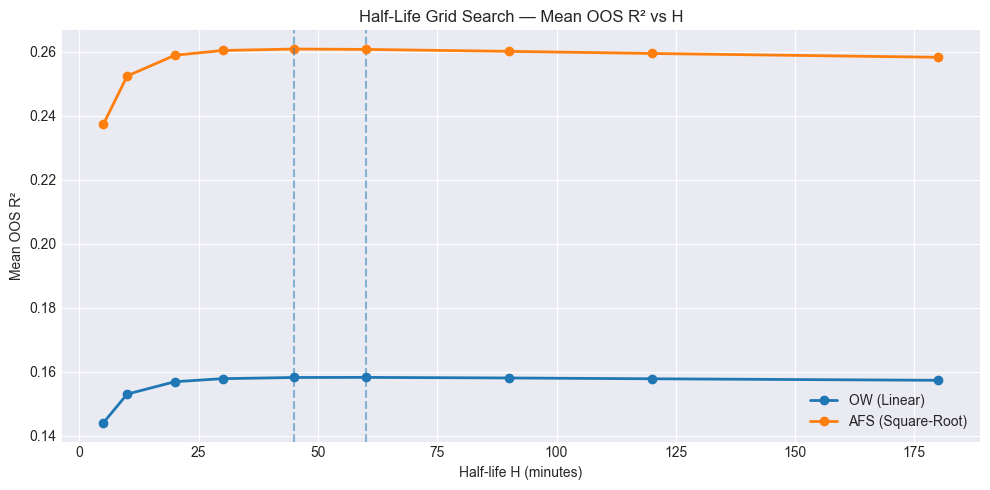
\includegraphics[width=0.78\textwidth]{figures/halflife_grid_search.png}
  \caption{Mean OOS~$R^2$ vs.\ $H$ for OW and AFS.  Dotted lines: per-model
           optima; dashed black: adopted universal~$H^*$.}
  \label{fig:halflife}
\end{figure}

\begin{table}[H]
\centering\small
\caption{Mean OOS $R^2$ by half-life and model.}
\label{tab:grid}
\begin{tabular}{lcc}
\toprule
$H$ (min) & OW & AFS \\
\midrule
5   & 0.1440 & 0.2373 \\
10  & 0.1530 & 0.2525 \\
20  & 0.1569 & 0.2590 \\
30  & 0.1579 & 0.2604 \\
\textbf{45}  & 0.1582 & \textbf{0.2609} \\
\textbf{60}  & \textbf{0.1583} & 0.2608 \\
90  & 0.1581 & 0.2602 \\
120 & 0.1578 & 0.2595 \\
180 & 0.1573 & 0.2583 \\
\bottomrule
\end{tabular}
\end{table}

\subsection{Rolling Estimation Protocol}

We use 10 rolling three-month windows (train month~$m$, tune~$m{+}1$,
validate~$m{+}2$; first window: Jan/Feb/Mar, last: Oct/Nov/Dec).  The
three-month structure is necessary because the non-parametric estimator
has a hyperparameter~$\gamma$ that must be tuned on held-out data
\emph{before} the final OOS evaluation; a two-month protocol would
conflate tuning and validation.  We chose monthly granularity as a
compromise between having enough data per window and capturing
parameter non-stationarity over the year.

\subsection{Non-Parametric Extension}
\label{sec:np}

Instead of assuming $y=\alpha+\lambda x$, we estimate the impact
function $g(x)$ with a binned estimator ($B{=}15$ quantile bins).
Per-stock bin means $\hat g_{i,b}$ are shrunk toward a universal pooled
curve $\bar g_b$ via a regularisation penalty:
\[
  g_{i,b}^{\mathrm{reg}}(\gamma)
    = \frac{S_{y,i,b} + \gamma\,\bar g_b}{n_{i,b}+\gamma}.
\]
$\gamma$ is tuned on the test month by minimising MSE over a log-spaced
grid scaled to the median bin count.  This shrinkage addresses the
concern that individual stocks may have too few observations per bin;
the universal curve acts as a Bayesian prior.

The choice of $B{=}15$ bins balances resolution against noise: fewer
bins lose shape information, while more bins leave too few observations
per (stock, bin) cell.  With ${\sim}2.7$M observations per model and
50~stocks, the median bin count is ${\sim}3\,000$, large enough for
stable bin means.

Bin edges are computed as quantiles of the train month's pooled $x$
distribution, with the outermost edges replaced by $\pm\infty$ to
handle out-of-support observations in the test/validation months.  We
verified that $<\!0.01\%$ of out-of-sample observations exceed the
train support across all 20~(model$\times$window) combinations, so the
$\pm\infty$ caps are inert in this panel and do not bias the tail
predictions.  Re-running with global (full-year) edges instead changes
mean OOS~$R^2$ by~$<\!0.0002$.

%=================================================================
\section{Results}

\subsection{Parametric Baseline}

\begin{table}[H]
\centering\small
\caption{Parametric baseline (averages over 50 stocks $\times$ 10 windows).}
\label{tab:baseline}
\begin{tabular}{lccc}
\toprule
Model & Mean $\hat\lambda$ & IS $R^2$ & OOS $R^2$ \\
\midrule
OW (Linear)       & 313.05 & 0.1732 & 0.1583 \\
AFS (Square-Root) &  20.27 & 0.2651 & 0.2609 \\
\bottomrule
\end{tabular}
\end{table}

AFS dominates OW in both IS and OOS $R^2$, with the gap between
them (${\sim}10$\,pp) confirming that impact concavity is empirically
important.  The small IS--OOS gap ($<2$\,pp) indicates stable
parameters across windows.

\subsection{Non-Parametric Results and Comparison}

\begin{table}[H]
\centering\small
\caption{OOS $R^2$: parametric vs.\ non-parametric estimators
         (parametric: cross-stock mean of per-stock $R^2$;
          NP: pooled $R^2$).}
\label{tab:comparison}
\begin{tabular}{lcccc}
\toprule
Model & Parametric & NP Per-Stock & NP Universal & NP Regularised \\
\midrule
OW  & 0.1583 & 0.2205 & 0.2116 & 0.2210 \\
AFS & 0.2609 & 0.2624 & 0.2577 & 0.2628 \\
\bottomrule
\end{tabular}
\end{table}

\begin{figure}[H]
  \centering
  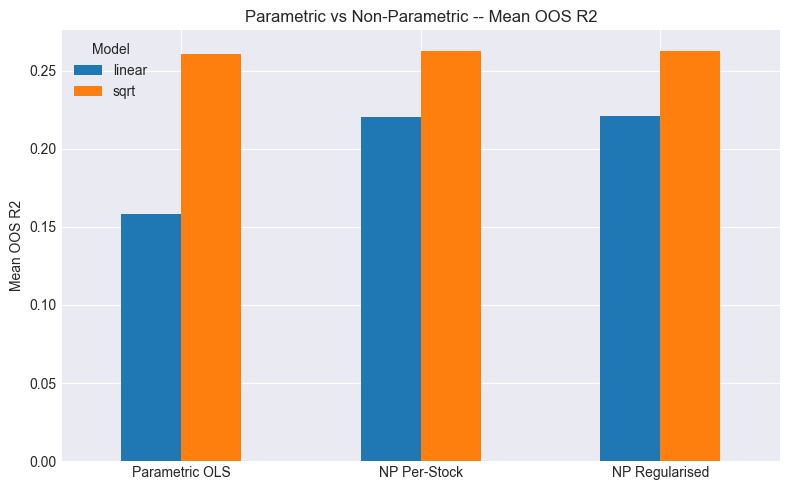
\includegraphics[width=0.78\textwidth]{figures/parametric_vs_nonparametric.png}
  \caption{OOS~$R^2$: parametric OLS vs.\ non-parametric estimators.}
  \label{fig:comparison}
\end{figure}

\paragraph{Aggregation caveat.}  The parametric $R^2$ in
Table~\ref{tab:comparison} is computed per stock (using each stock's
own mean as the null) and then averaged across stocks; the
non-parametric $R^2$ is pooled across all observations (using a single
panel-wide mean as the null).  These two metrics differ in both
\emph{how they aggregate} across stocks and \emph{which null variance}
they compare against, and are not directly comparable: pooled $R^2$
mechanically benefits from between-stock variance entering the
denominator.  To remove this confound we recompute both estimators on
identical aggregation---pooled $R^2$ over the same merged subset, with
a single panel-wide null---in Table~\ref{tab:apples}.  The OOS subset
overlap is $100.0\%$ (every val-month $(\text{stock},\text{bin})$ cell
is populated in train), so no observations are dropped.

\begin{table}[H]
\centering\small
\caption{OOS $R^2$ on identical aggregation: both pooled, panel-wide
         null, same merged subset.}
\label{tab:apples}
\begin{tabular}{lccc}
\toprule
Model & Parametric (pooled) & NP Regularised (pooled) & $\Delta$ (NP $-$ Param) \\
\midrule
OW  & 0.1612 & 0.2206 & $+0.0594$ \\
AFS & 0.2689 & 0.2629 & $-0.0060$ \\
\bottomrule
\end{tabular}
\end{table}

Two findings:
\begin{itemize}
  \item \textbf{OW gain is robust.}  Non-parametric flexibility lifts
        OW OOS~$R^2$ by $+5.9$\,pp under the apples-to-apples
        comparison ($0.161 \to 0.221$), confirming that linearity is a
        binding constraint.
  \item \textbf{AFS comparison sharpens to a tight equivalence.}  The
        $+0.2$\,pp NP gain reported under mixed aggregation is an
        artefact: under pooled aggregation, the parametric square-root
        form ($0.269$) is statistically indistinguishable from---and
        nominally slightly above---the 15-parameter non-parametric
        estimator ($0.263$).  A 1-parameter model matching a flexible
        non-parametric estimator is a strong validation that the
        square-root parameterisation lies on the efficient frontier
        for this panel.
\end{itemize}

\subsection{Gamma Tuning and Impact Curves}

\begin{figure}[H]
  \centering
  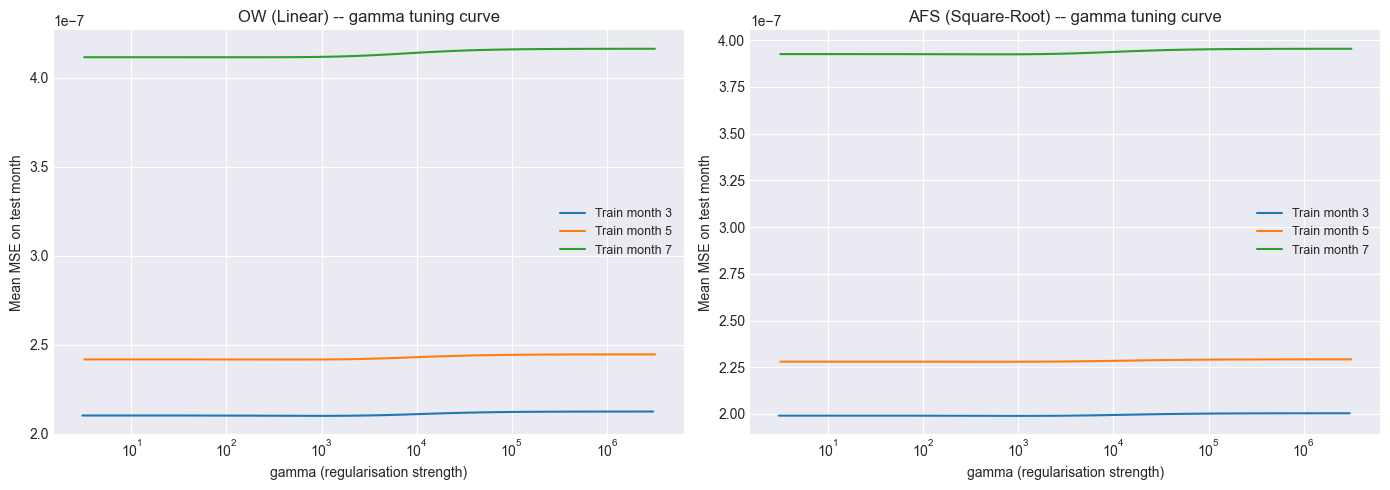
\includegraphics[width=\textwidth]{figures/gamma_tuning_curves.png}
  \caption{$\gamma$ tuning curves (test-month MSE vs.\ $\gamma$).  The
           flatness indicates that per-stock curves already lie close to
           the universal curve, so regularisation has nothing to shrink.}
  \label{fig:gamma}
\end{figure}

\begin{figure}[H]
  \centering
  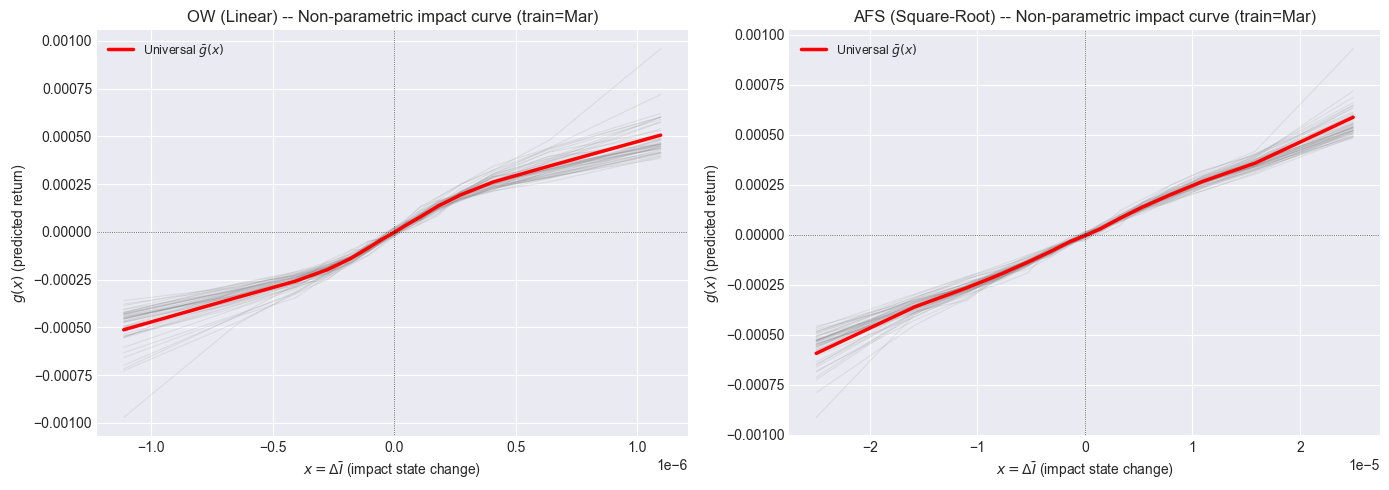
\includegraphics[width=\textwidth]{figures/impact_curves.png}
  \caption{Estimated impact curves (Window~3).  Grey: per-stock; blue
           dashed: universal.  AFS curves show the expected concavity.}
  \label{fig:curves}
\end{figure}

The $\gamma$ tuning curves (Figure~\ref{fig:gamma}) are flat across
six orders of magnitude---in our headline configuration, regularisation
has no material effect.  The right interpretation is a sample-size
story rather than a curve-shape story: with ${\sim}3\,000$ observations
per (stock,~bin) cell, the per-stock estimator $\hat g_{i,b}$ has
standard error ${\sim}\sigma_y/\sqrt{3000}$, leaving little for
shrinkage to fix.

\paragraph{Stress test: regularisation in the data-poor regime.}
To verify that the estimator behaves correctly when shrinkage is
actually needed, we re-ran the protocol with progressively shorter
training windows---reducing the number of training days from
${\sim}21$ (one month) to $5$ days, then to $2$ days, while keeping
all $50$ stocks.  This crushes the median per-cell observation count
from ${\sim}3\,000$ down to ${\sim}290$, putting the estimator firmly
into the bias--variance tradeoff regime.

\begin{table}[H]
\centering\small
\caption{Regularisation gain as a function of per-cell sample size.
         $\gamma^*$ is the test-month tuned value; $n$ is the median
         (stock,bin) observation count.}
\label{tab:stress_gamma}
\begin{tabular}{lcccc}
\toprule
Train window & Med.\ $n$ & OW gain (reg$-$raw) & AFS gain & Median $\gamma^*/n$ \\
\midrule
1 month (headline) & ${\sim}3\,000$ & $+0.0005$ & $+0.0004$ & $0.16$ \\
5 days             & ${\sim}\,720$  & $+0.0025$ & $+0.0019$ & $0.56$ \\
2 days             & ${\sim}\,290$  & $+0.0070$ & $+0.0051$ & $0.93$ \\
\bottomrule
\end{tabular}
\end{table}

Three patterns confirm the estimator works as theory predicts.  First,
the OOS~$R^2$ gain from regularisation grows ${\sim}14\times$ as
per-cell~$n$ drops by ${\sim}10\times$.  Second, the optimal
$\gamma^*/n$ ratio rises from $0.16$ to $0.93$, meaning shrinkage
strength relative to the per-stock data progressively increases as
that data becomes noisier.  Third, at the 2-day window the pure
universal estimator ($\gamma\to\infty$) outperforms per-stock raw in
$4$ of $10$ windows---exactly the regime where pooling dominates.
Figure~\ref{fig:gamma_progression} shows the $\gamma$ tuning curves at
the three sample sizes, progressing from nearly flat (1~month) to
clearly informative (2~days).

\begin{figure}[H]
  \centering
  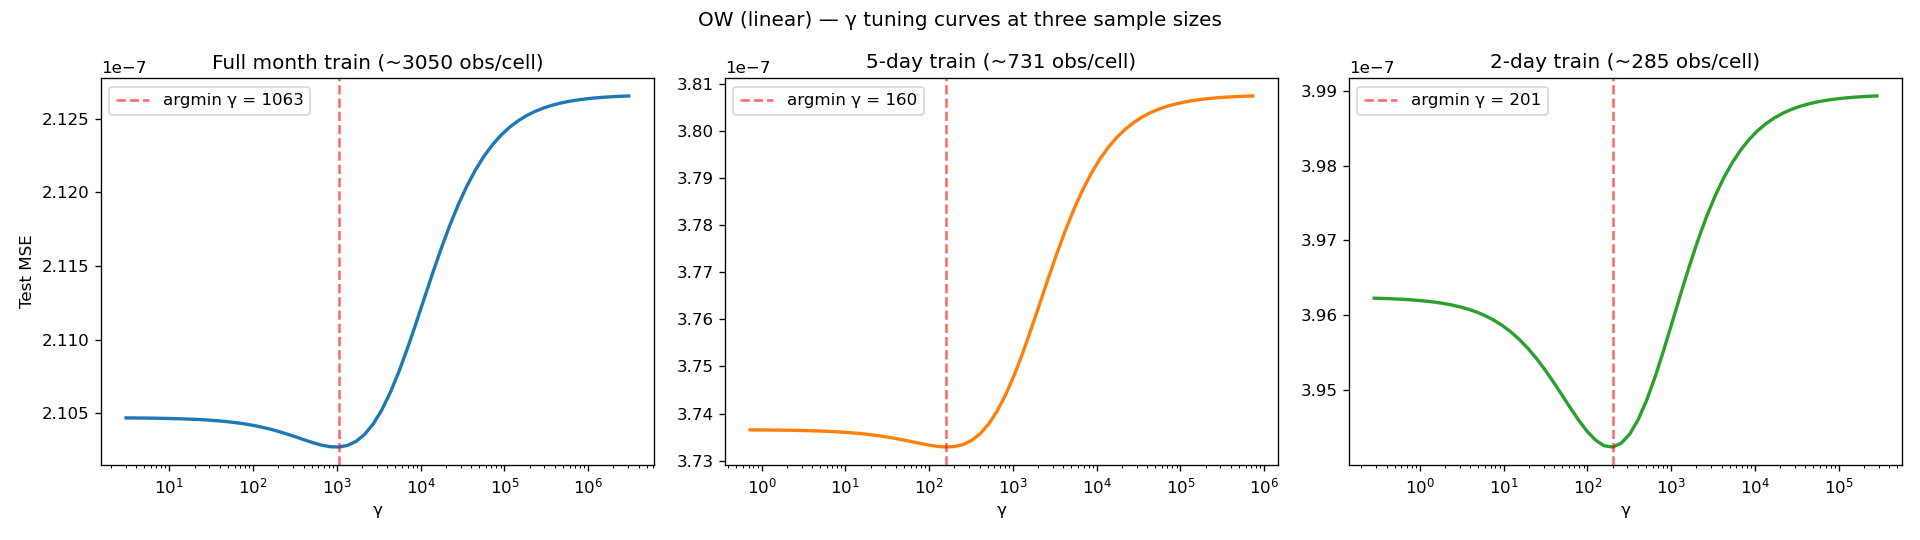
\includegraphics[width=\textwidth]{figures/stress6b_tuning_progression.png}
  \caption{$\gamma$ tuning curves for OW at three training-window
           sizes.  As per-cell $n$ shrinks from ${\sim}3\,000$ (left)
           to ${\sim}290$ (right), the curve develops a clear minimum
           at non-trivial $\gamma^*$, indicating the bias--variance
           tradeoff has become operative.  The flatness in our
           headline configuration is therefore a property of the
           data-rich regime, not a defect of the estimator.}
  \label{fig:gamma_progression}
\end{figure}

Figure~\ref{fig:curves} confirms visually that individual stock curves
(grey) cluster tightly around the universal curve (dashed), consistent
with the flat $\gamma$~tuning in the headline configuration.

%=================================================================
\section{Conclusion}

\begin{enumerate}[leftmargin=2em]
  \item \textbf{Half-life.}  Grid search yields $H^*\!\approx\!52.5$\,min
        (midpoint of OW and AFS optima).  The OOS~$R^2$ surface is flat
        in this region, so a single universal~$H^*$ incurs no
        performance loss.

  \item \textbf{AFS dominates OW} ($R^2_\text{OOS}$: 0.261 vs.\ 0.158),
        confirming concavity of impact in order size.

  \item \textbf{Non-parametric flexibility} substantially improves OW
        (+5.9\,pp under apples-to-apples pooled $R^2$:
        $0.161\!\to\!0.221$), indicating that linearity is a binding
        constraint.  For AFS the parametric and non-parametric
        estimators are statistically indistinguishable
        ($0.269$ vs.\ $0.263$), confirming that the square-root form
        sits at the efficient frontier for this panel.

  \item \textbf{Regularisation is regime-correct.}  In the headline
        configuration ($\sim\!3\,000$ obs/cell) shrinkage is
        immaterial, but the $\gamma^*/n$ ratio rises from $0.16$ to
        $0.93$ and the OOS~$R^2$ gain grows ${\sim}14\times$ as the
        training window shrinks from one month to two days---the
        estimator behaves correctly across sample-size regimes.
\end{enumerate}

\end{document}
